\chapter{Metodología}
\label{cap:metodologia}

En este apartado se va a describir la metodología utilizada durante la realización de este proyecto. A su vez, se va a incluir una descripción de las herramientas, tecnologías y técnicas usadas, asi como de una justificación de dichas elecciones.

\section{Metodología}

La metodología seguida puede considerarse como \textit{Scrum}.\\

Al comienzo de este proyecto se tuvieron varias reuniones para establecer los objetivos y requisitos que debía de cumplir este proyecto, aunque no en demasiada profundidad, siendo esto una tarea que se llevo a cabo según lo establecido en el capítulo anterior.\\

Una vez finalizadas dichas reuniones iniciales, se establecieron una serie de fechas en las cuales se tuvieron otras reuniones para comprobar el estado del proyecto. Estas fechas coinciden con la planificiación. Para cada reunión, se establecía una serie de objetivos que se debían alcanzar para el correcto desarrollo del proyecto y garantizar que se cumplía con la planificación establecida. De esta manera, se intercambiaron opiniones sobre la situación del proyecto, comentando posibles mejoras y solucionando las dudas surgidas durante las distintas etapas del desarrollo.\\

\section{Herramientas usadas}

En esta sección vamos a comentar las herramientas que han sido usadas durante la realización del proyecto.

\subsection{Android Studio}

Aunque no es estrictamente necesario para desarrollar aplicaciones Android, es posible utilizar eclipse por ejemplo, he decidio usarlo ya que es muy sencillo de entender y facilita al progamador muchas tareas. Esto ha sido muy importante ya que, como he comentado antes, mi experiencia con Android era muy reducida.\\

Android Studio es el entorno de desarrollo integrado, \textit{IDE}, oficial para la plataforma Android. Por esta razón la documentación es abundante, lo que supone un gran punto a su favor.\\

\begin{figure}[H] %con el [H] le obligamos a situar aquí la figura
\centering
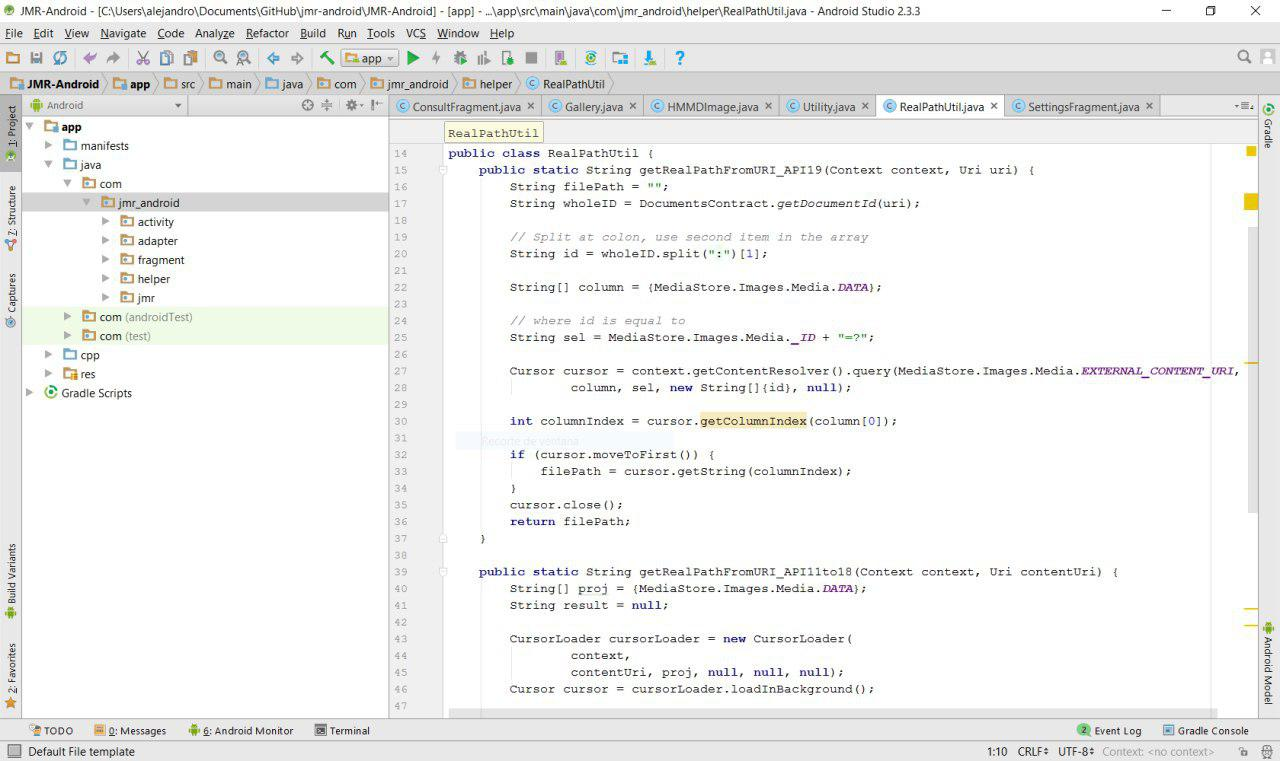
\includegraphics[scale=0.5]{imagenes/android-studio.jpg}  %el parámetro scale permite agrandar o achicar la imagen. En el nombre de archivo puede especificar directorios
\label{android-studio.jpg}
\caption{Ejemplo de proyecto Android Studio}
\end{figure}

Otra de las cosas interesantes de este \textit{IDE} es la posibilidad de diseñar interfaces de una manera muy sencilla e intuitiva, permitiendo arrastar los elementos a las posiciones deseadas. Por lo que no se requiere un gran nivel de programación para estas tareas. Aunque si hay que comentar, que si se necesita hacer cosas más complicadas, o que no sean las estándar, si es necesario un nivel de programación avanzado, ya que en dicho caso, la ayuda proporcionada por Android Studio para estas tareas se reduce.\\ 

\subsection{Git y GitHub}

Al tratarse de un proyecto de esta magnitud, ha sido necesario utilizar una herramienta de control de versiones, como es natural se ha utilizado git.\\

También se ha usado GitHub, que se trata de un lugar donde alojar nuestros proyectos utilizando el sistema de control de versiones Git. Por lo tanto, podemos entender que git y GitHub van de la mano, al menos en este caso.\\

El respositorio del proyecto se puede consultar \href{https://github.com/acasadoquijada/jmr-android}{aquí}.

Para llevar un control del proyecto se han usado los elementos conocidos como \textit{Milestones} y \textit{Issues} por GitHub.\\

Podemos entender un \textit{Issue} como una tarea por realizar, siendo un ejemplo, \textit{seleccionar imagen de la galería}. Se les puede añadir información extra, como a que \textit{Milestone} está asociado, que persona es la encargada de solucionarlo, o se puede añadir una etiqueta para establecer el tipo.\\

\begin{figure}[H] %con el [H] le obligamos a situar aquí la figura
\centering
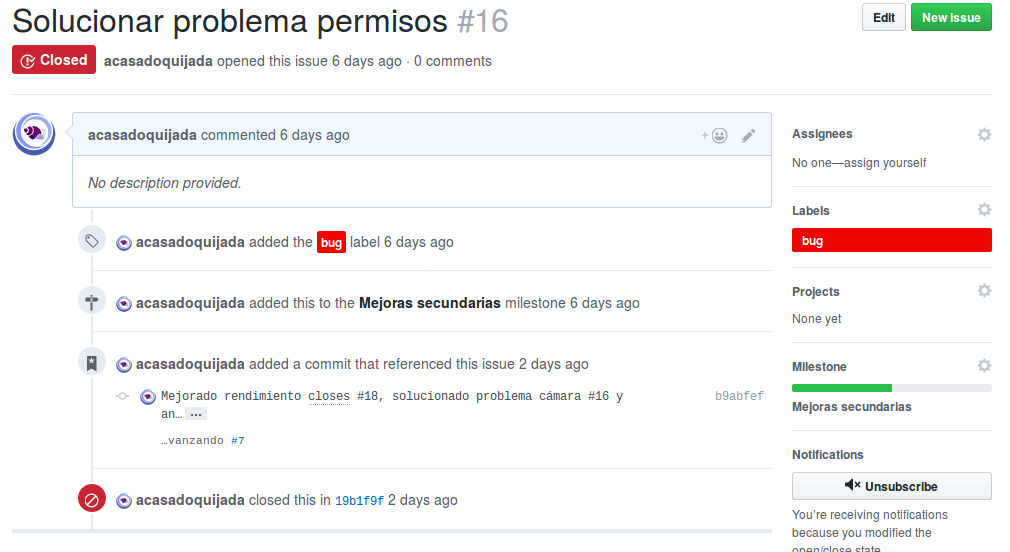
\includegraphics[scale=0.4]{imagenes/issue.png}  %el parámetro scale permite agrandar o achicar la imagen. En el nombre de archivo puede especificar directorios
\label{issue.png}
\caption{Ejemplo de issue}
\end{figure}

Por otro lado, se encuentran los \textit{Milestones}, que podemos considerarlos como hitos, es decir, un \textit{Milestone} está compuesto por varios \textit{Issues}. Por lo que también puede ser vistos como una agrupación de \textit{Issues}, una gran tarea dividida en pequeñas subtareas.\\

\begin{figure}[H] %con el [H] le obligamos a situar aquí la figura
\centering
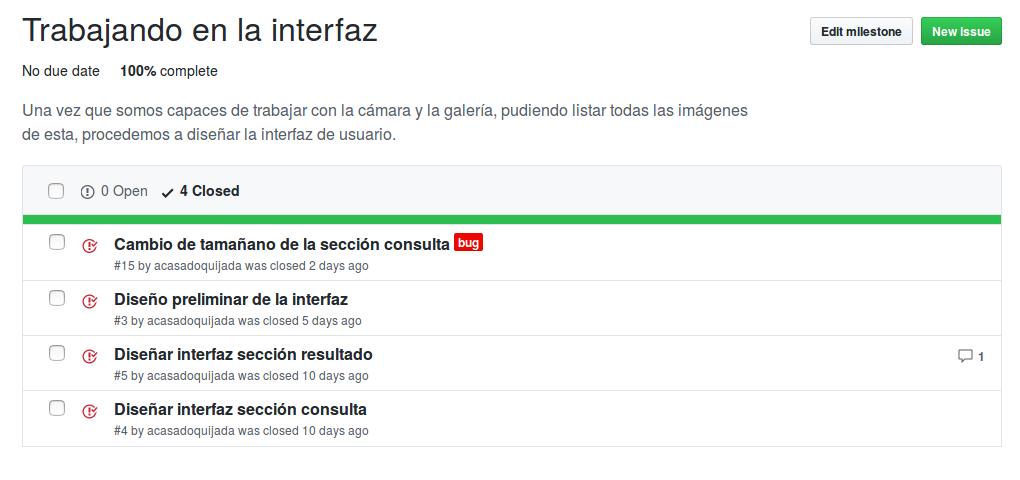
\includegraphics[scale=0.4]{imagenes/milestone.png}  %el parámetro scale permite agrandar o achicar la imagen. En el nombre de archivo puede especificar directorios
\label{milestone.png}
\caption{Ejemplo de milestone}
\end{figure}

Como se puede entender, usar ambos es de vital importancia si se desea llevar a cabo un proyecto de gran magnitud.

\subsection{Dispotivio de pruebas}

Aunque Android Studio nos ofrece la posibilidad de utilizar un emulador para lanzar la apliación, he decidido utilizar mi dispositivo móvil, por motivos de eficiencia y comodidad. Debido a que no se podía comprobar de manera real algunos aspectos de la propia aplicación, como el consumo de memoria o el propio rendimiento de las consultas.\\

Mi smartphone es un \textit{Xiaomi redmi 4 pro}, y cuenta con las siguientes características destacables:

\begin{itemize}
\item CPU: Qualcomm Snapdragon 625, con ocho núcleos y 2GHz 
\item Memoria: 3 GB
\item Almacenamiento: 32 GB
\end{itemize}

Se tratan de unas características que suelen ser habituales de encontrar en los smartphones actuales, por lo que ha sido un gran sujeto de pruebas.

\section{Tecnicas}

Para programar en Android se utiliza \textit{Java} para la lógica, y \textit{XML} para las interfaces de usuario.\\

Como es habitual, el desarrollo en Java ha seguido un paradigma de programación orientada a objetos, \textit{POO}. En el que se han desarrollado una serie de clases que se han organizado en distintos paquetes. Esto será explicado posteriormente.\\ 

Comentar que se ha utilizado también \textit{Android NDK}. Se trata de un conjunto de herramientas que nos permiten implementar partes de la aplicación en código nativo, como \textit{C} o \textit{C++}. Esta opción es perfecta para usar en los cálculos que realiza la aplicación. Como en el caso anterior se comentará con más detalle en su correspondiente sección.\\

\begin{figure}[H] %con el [H] le obligamos a situar aquí la figura
\centering
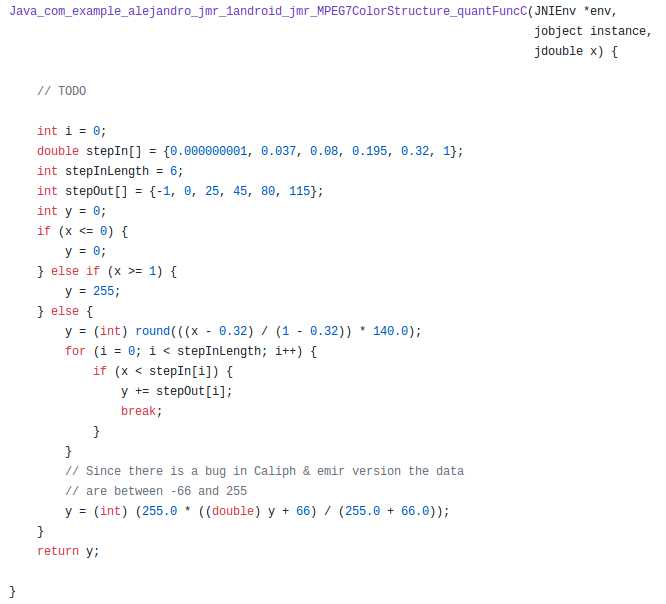
\includegraphics[scale=0.6]{imagenes/ndk.png}  %el parámetro scale permite agrandar o achicar la imagen. En el nombre de archivo puede especificar directorios
\label{ndk.png}
\caption{Ejemplo de código Android ndk}
\end{figure}

Por último comentar que se ha usado \textit{XML} para las interfaces de usuario, la mayor parte del tiempo apoyándose en el soporte proporcionado por Android Studio, pero que a la hora de realizar cosas mas complejas se ha tenido que escribir manualmente dicho código XML.

\begin{figure}[H] %con el [H] le obligamos a situar aquí la figura
\centering
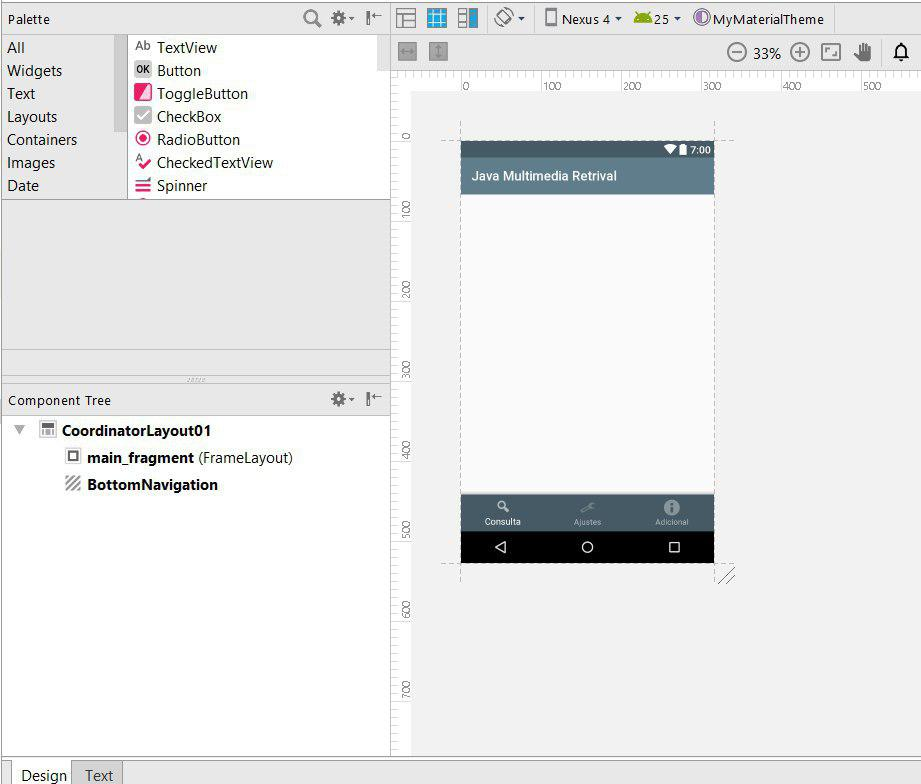
\includegraphics[scale=0.6]{imagenes/interfaz-android-studio.jpg}  %el parámetro scale permite agrandar o achicar la imagen. En el nombre de archivo puede especificar directorios
\label{interfaz-android-studio.jpg}
\caption{Ejemplo de proyecto Android Studio}
\end{figure}

\section{Historias de usuario}

Cuando nos referimos a historias de usuario, nos refererimos a la representación de un requisito que se encuentra escrito en varias frases cortas, utilizando el lenguaje común del usuario. Esto facilita la comprensión y realización de los requisitos de un proyecto.\\

En este caso se apoyan fuertemente en los objetivos que se establecieron al comienzo de la memoría.\\

A continuación vamos a comentar las historias de usuario correspondientes a este proyecto.

\begin{table}[H]
	\begin{center}
		\begin{tabular} {l|c|l}
			\hline
			1 & \multicolumn{2}{c}{Interacción con la interfaz} \\ \noalign{\hrule height 1pt}
			\multicolumn{3}{l}{Descripción} \\ \hline
			\multicolumn{3}{p{12cm}}{Se podra mover con libertad por los distintos menús diponibles en la interfaz.} \\ \noalign{\hrule height 1pt}
			\multicolumn{3}{l}{Pruebas de aceptación} \\ \hline
			\multicolumn{3}{p{12cm}}{ - Comprobar que al pulsar en al pulsar el item \textbf{consulta} se muestra la interfaz asociada.} \\
			\multicolumn{3}{p{12cm}}{ - Comprobar que al pulsar en el action button, este se despliega mostrando dos opciones, cámara y galería.} \\
			\multicolumn{3}{p{12cm}}{ - Comprobar que al pulsar en al pulsar el item \textbf{ajustes} se muestra la interfaz asociada.} \\ \hline
			\multicolumn{3}{p{12cm}}{ - Comprobar que al pulsar en al pulsar el item \textbf{adicional} se muestra la interfaz asociada.} \\ 
			\hline
		\end{tabular}
	\end{center}
	\caption{Historia de usuario - Interacción con la interfaz}
	\label{tab:interaccion-interfaz}
\end{table}

\begin{table}[H]
	\begin{center}
		\begin{tabular} {l|c|l}
			\hline
			2 & \multicolumn{2}{c}{Cargar imagen cámara} \\ \noalign{\hrule height 1pt}
			\multicolumn{3}{l}{Descripción} \\ \hline
			\multicolumn{3}{p{12cm}}{Se podra mover cargar la imagen consulta utilizando la cámara del dispositivo.} \\ \noalign{\hrule height 1pt}
			\multicolumn{3}{l}{Pruebas de aceptación} \\ \hline
			\multicolumn{3}{p{12cm}}{ - Comprobar que al pulsar en al pulsar el item \textbf{cámara} del \textit{floating button}, se lanza la actividad cámara, pudiendo elegir la delantera o trasera en caso de que se diponga de ellas.} \\
			\multicolumn{3}{p{12cm}}{ - Comprobar que al tomar una fotografía esta se añade a la sección de imágenes consulta.} \\
			\multicolumn{3}{p{12cm}}{ - Comprobar que al pulsar en al pulsar en el item \textbf{consultar}, se realiza la consulta con esta nueva imagen.} \\ \hline
		\end{tabular}
	\end{center}
	\caption{Historia de usuario - Cargar imagen consulta cámara}
	\label{tab:interaccion-interfaz}
\end{table}

\begin{table}[H]
	\begin{center}
		\begin{tabular} {l|c|l}
			\hline
			3 & \multicolumn{2}{c}{Cargar imagen galería} \\ \noalign{\hrule height 1pt}
			\multicolumn{3}{l}{Descripción} \\ \hline
			\multicolumn{3}{p{12cm}}{Se podra mover cargar la imagen consulta utilizando la galería del dispositivo.} \\ \noalign{\hrule height 1pt}
			\multicolumn{3}{l}{Pruebas de aceptación} \\ \hline
			\multicolumn{3}{p{12cm}}{ - Comprobar que al pulsar en al pulsar el item \textbf{galería} del \textit{floating button}, se lanza la galería.} \\
			\multicolumn{3}{p{12cm}}{ - Comprobar que al tomar seleccionar una imagen, esta se añade a la sección de imágenes consulta.} \\
			\multicolumn{3}{p{12cm}}{ - Comprobar que al pulsar en al pulsar en el item \textbf{consultar}, se realiza la consulta con esta nueva imagen.} \\ \hline
		\end{tabular}
	\end{center}
	\caption{Historia de usuario - Cargar imagen consulta galería}
	\label{tab:interaccion-interfaz}
\end{table}

\begin{table}[H]
	\begin{center}
		\begin{tabular} {l|c|l}
			\hline
			4 & \multicolumn{2}{c}{Realizar consulta} \\ \noalign{\hrule height 1pt}
			\multicolumn{3}{l}{Descripción} \\ \hline
			\multicolumn{3}{p{12cm}}{Se podra mover realizar una consulta usando una de las fotos consulta.} \\ \noalign{\hrule height 1pt}
			\multicolumn{3}{l}{Pruebas de aceptación} \\ \hline
			\multicolumn{3}{p{12cm}}{ - Comprobar que al pulsar durante unos segundos sobre una imagen esta se establece como la imagen consulta.} \\
			\multicolumn{3}{p{12cm}}{ - Comprobar que solo una imagen puede ser seleccionada para su consulta al mismo tiempo.} \\
			\multicolumn{3}{p{12cm}}{ - Comprobar que al pulsar en al pulsar en el item \textbf{consultar}, se realiza la consulta con esta imagen seleccionada.} \\ \hline
		\end{tabular}
	\end{center}
	\caption{Historia de usuario - Realizar consulta}
	\label{tab:interaccion-interfaz}
\end{table}

\begin{table}[H]
	\begin{center}
		\begin{tabular} {l|c|l}
			\hline
			5 & \multicolumn{2}{c}{Cambiar de descriptor} \\ \noalign{\hrule height 1pt}
			\multicolumn{3}{l}{Descripción} \\ \hline
			\multicolumn{3}{p{12cm}}{Se podra cambiar el descriptor que se emplea durante las consultas.} \\ \noalign{\hrule height 1pt}
			\multicolumn{3}{l}{Pruebas de aceptación} \\ \hline
			\multicolumn{3}{p{12cm}}{ - Comprobar que al pulsar sobre el descriptor deseado este queda maracado como activo.} \\
			\multicolumn{3}{p{12cm}}{ - Comprobar que solo un descriptor puede ser seleccionado.} \\
			\multicolumn{3}{p{12cm}}{ - Comprobar que al pulsar en al pulsar en el item \textbf{consultar}, se realiza la consulta con este descriptor seleccionado.} \\ \hline
		\end{tabular}
	\end{center}
	\caption{Historia de usuario - Cambiar descriptor}
	\label{tab:interaccion-interfaz}
\end{table}

\begin{table}[H]
	\begin{center}
		\begin{tabular} {l|c|l}
			\hline
			6 & \multicolumn{2}{c}{Eliminar base de datos} \\ \noalign{\hrule height 1pt}
			\multicolumn{3}{l}{Descripción} \\ \hline
			\multicolumn{3}{p{12cm}}{Se podra eliminar la base de datos.} \\ \noalign{\hrule height 1pt}
			\multicolumn{3}{l}{Pruebas de aceptación} \\ \hline
			\multicolumn{3}{p{12cm}}{ - Comprobar que al pulsar sobre la opción \textit{Eliminar BD} se lanza un desplegable para realizar la acción.} \\
			\multicolumn{3}{p{12cm}}{ - Comprobar que al pulsar en aceptar, se notifica de que la BD ha sido eliminada.} \\
		\end{tabular}
	\end{center}
	\caption{Historia de usuario - Eliminar base de datos}
	\label{tab:interaccion-interfaz}
\end{table}

\begin{table}[H]
	\begin{center}
		\begin{tabular} {l|c|l}
			\hline
			7 & \multicolumn{2}{c}{Calcular base de datos} \\ \noalign{\hrule height 1pt}
			\multicolumn{3}{l}{Descripción} \\ \hline
			\multicolumn{3}{p{12cm}}{Se podra precalcular la base de datos para agilizar consultas.} \\ \noalign{\hrule height 1pt}
			\multicolumn{3}{l}{Pruebas de aceptación} \\ \hline
			\multicolumn{3}{p{12cm}}{ - Comprobar que al pulsar sobre la opción \textit{Calcular BD} se lanza un diálogo sobre el proceso.} \\
			\multicolumn{3}{p{12cm}}{ - Comprobar que al realizar una consulta, el tiempo es menor que si no hubiese base de datos.} \\
		\end{tabular}
	\end{center}
	\caption{Historia de usuario - Calcular base de datos}
	\label{tab:interaccion-interfaz}
\end{table}

\begin{table}[H]
	\begin{center}
		\begin{tabular} {l|c|l}
			\hline
			8 & \multicolumn{2}{c}{Elegir número de imágenes} \\ \noalign{\hrule height 1pt}
			\multicolumn{3}{l}{Descripción} \\ \hline
			\multicolumn{3}{p{12cm}}{Se podra elegir el número de imágenes que serán consultadas.} \\ \noalign{\hrule height 1pt}
			\multicolumn{3}{l}{Pruebas de aceptación} \\ \hline
			\multicolumn{3}{p{12cm}}{ - Comprobar que al pulsar sobre la opción \textit{Elegir número de imagenes} se lanza un desplegable permitiendonos elegir el número.} \\
			\multicolumn{3}{p{12cm}}{ - Comprobar que el número de las imágenes resultado se corresponde con el establecido previamente.} \\
		\end{tabular}
	\end{center}
	\caption{Historia de usuario - Elegir número de imágenes}
	\label{tab:interaccion-interfaz}
\end{table}

\begin{table}[H]
	\begin{center}
		\begin{tabular} {l|c|l}
			\hline
			9 & \multicolumn{2}{c}{Interactuar con las imágenes consulta} \\ \noalign{\hrule height 1pt}
			\multicolumn{3}{l}{Descripción} \\ \hline
			\multicolumn{3}{p{12cm}}{Se podra interactuar con las imágenes consulta.} \\ \noalign{\hrule height 1pt}
			\multicolumn{3}{l}{Pruebas de aceptación} \\ \hline
			\multicolumn{3}{p{12cm}}{ - Comprobar que se puede realizar movimiento scroll de derecha a izquierda y viceversa sobre las imágenes consulta, siempre que haya las suficientes.} \\
			\multicolumn{3}{p{12cm}}{ - Comprobar que al pulsar sobre una, esta se muestra a pantalla completa indicándonos la posición que ocupa respecto a las demás.} \\
		\end{tabular}
	\end{center}
	\caption{Historia de usuario - Interactuar con las imágenes consulta }
	\label{tab:interaccion-interfaz}
\end{table}

\begin{table}[H]
	\begin{center}
		\begin{tabular} {l|c|l}
			\hline
			10 & \multicolumn{2}{c}{Interactuar con las imágenes resultado} \\ \noalign{\hrule height 1pt}
			\multicolumn{3}{l}{Descripción} \\ \hline
			\multicolumn{3}{p{12cm}}{Se podra interactuar con las imágenes resultado.} \\ \noalign{\hrule height 1pt}
			\multicolumn{3}{l}{Pruebas de aceptación} \\ \hline
			\multicolumn{3}{p{12cm}}{ - Comprobar que se puede realizar movimiento scroll hacia arriba, hacia abajo y viceversa sobre las imágenes resultado, siempre que haya las suficientes.} \\
			\multicolumn{3}{p{12cm}}{ - Comprobar que al pulsar sobre una, esta se muestra a pantalla completa indicándonos la posición que ocupa respecto a las demás, y la distancia respecto a la imagen consulta.} \\
		\end{tabular}
	\end{center}
	\caption{Historia de usuario - Interactuar con las imágenes consulta}
	\label{tab:interaccion-interfaz}
\end{table}
